\chapter{Tracing and Metrics}
\label{cap:tracing-metrics}

%%%%%%%%%%%%%%%%%%%%%%%%%%%%%%%%%%%%%%%%%%%%%%%%%%
\section{Tracing}
\label{cap:tracing}
In applicazioni con migliaia di micro servizi, seguire la cascata di chiamate o valutare in che punto si è verificato un errore è molto complesso. Tramite il tracing non solo possiamo capire quale micro servizio viene chiamato e da chi, ma possiamo anche analizzare i tempi con cui ogni richiesta è stata servita, sia E2E che all'interno del singolo servizio.

Il funzionamento solitamente è abbastanza semplice: durante le varie chiamate viene trasmesso anche un ID (univoco) della traccia; il trasporto di questo ID avviene tramite una qualche funzionalità del protocollo di trasporto, che in HTTP è il relativo header.

\subsection{OpenTelemetry}
OpenTelemetry, noto anche come OTel, è un insieme di tool e API che permette di collezionare ed esportare le telemetrie di un'applicazione a micro servizi. Oltre alle telemetrie in realtà possono anche essere gestite metriche e logs, ma in questo campo non è stabile e si preferisce usare altro (e.g., MicroMeter).

\myskip

Fornisce un protocollo, detto OTLP, che permette di esportare le telemetrie dalle applicazioni verso il tool OpenTelemetry Collector. A quest'ultimo si possono collegare vari back end (e.g., Jaeger) per la loro visualizzazione.

Usare il Collector non è necessario: si possono inviare i dati direttamente al backend: in piccole applicazioni è forse una scelta migliore per la facilità di manutenzione e configurazione; se l'applicazione deve scalare allora si hanno numero vantaggi usando il Collector, come il filtraggio, il batching e la riprova in caso di un qualche fallimento.

\myskip

Per utilizzare OTel nei vari micro servizi della nostra applicazione si deve semplicemente aggiungere l'estensione \textit{quarkus-opentelemetry}. In questo modo Quarkus inizia a collezionare telemetrie in automatico.

\subsection{Jaeger}
Come abbiamo detto Jaeger è un backend per la visualizzazione della cascate di chiamate all'interno di un applicazione a micro servizi.

Per permettere il suo funzionamento si deve aggiungere delle configurazioni nel file \textit{application.properties}. Queste configurazioni sono abbastanza standard e non dipendono molto dal microservizio specifico, se non per il nome che vogliamo visualizzare nella UI. Un esempio è quanto configurato per \textit{users-service} all'interno del Listing~\ref{lst:users-jaeger}. L'unica configurazione da spiegare è forse \texttt{quarkus.otel.traces.sampler=always\_on}: essa permette di non fare nessun campionamento delle chiamate, ma di considerarle e visualizzarle tutte; in questo modo non si rischia di interrompere una sequenza di chiamate.
\begin{lstlisting}[caption=Jaeger configuration for \textit{users-service}, label=lst:users-jaeger]
# jaeger
quarkus.otel.service.name=users-service
quarkus.otel.exporter.otlp.endpoint=http://jaeger-collector:4317
quarkus.otel.traces.sampler=always_on
\end{lstlisting}

\begin{figure}[htbp]
    \centering
    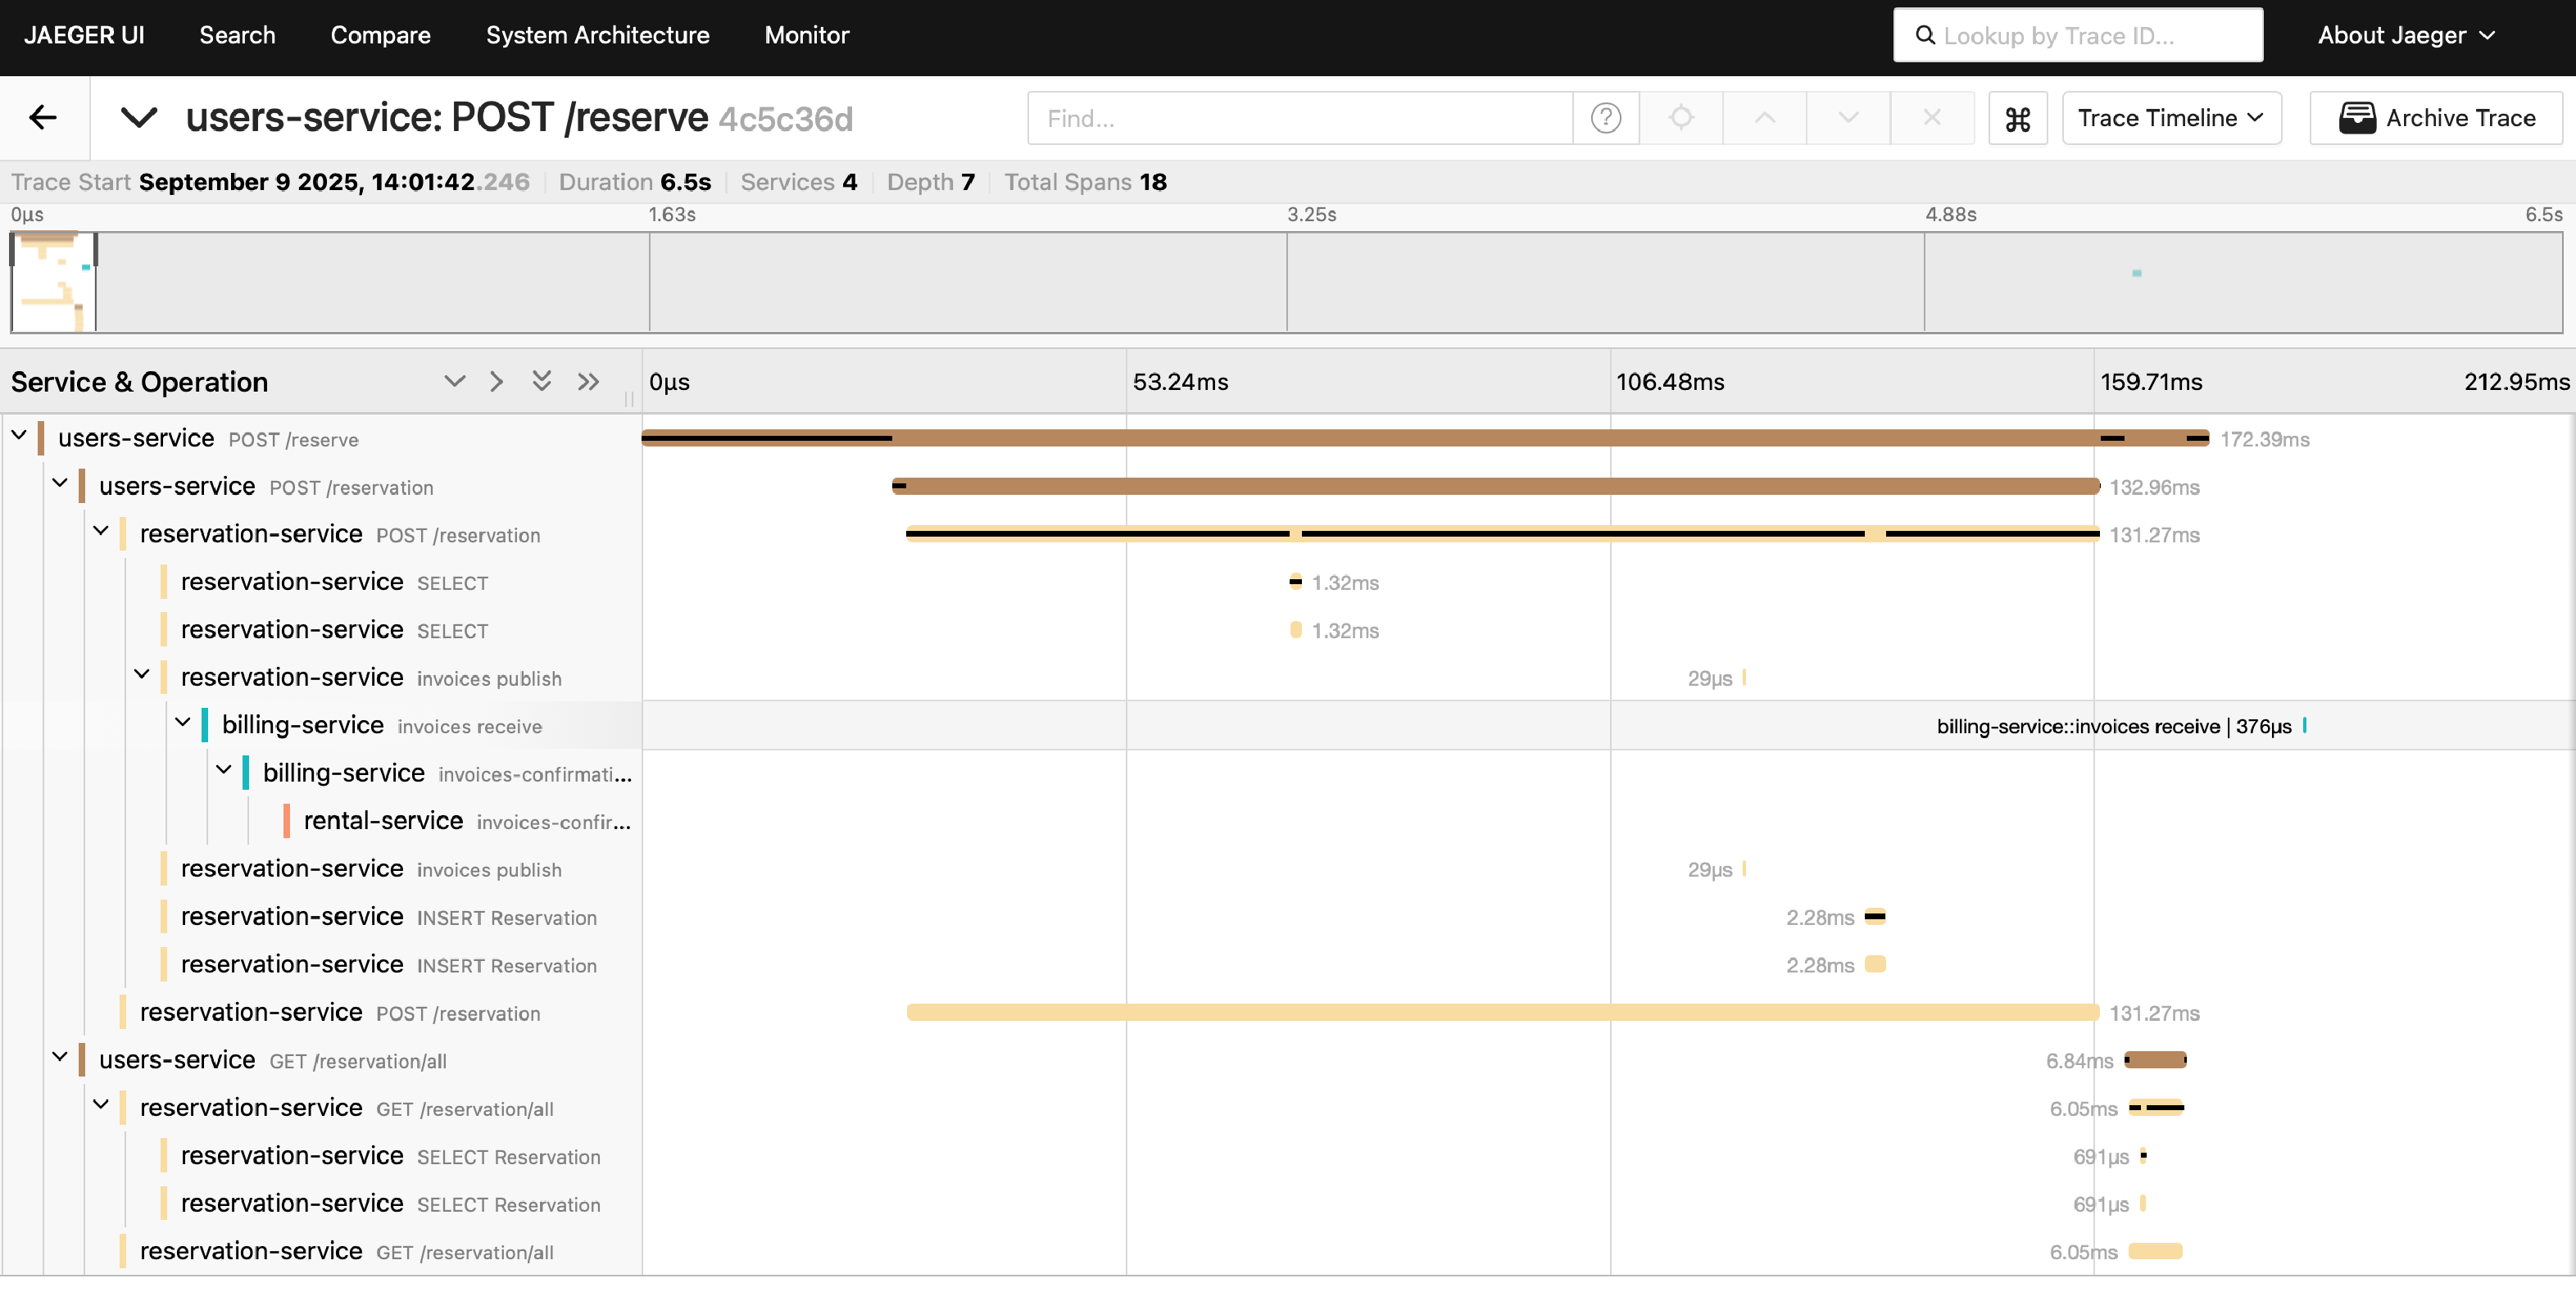
\includegraphics[width=.9\textwidth]{images/4-tracing_metrics/jaeger use case.pdf}
    \caption{Car resevation from user.}
    \label{fig:jaeger_reservation}
\end{figure}

\subsection{Jaeger deployment}
Come per i servizi terzi elencati nella Sezione~\ref{sec:servizi_esterni}, anche il backend Jaeger deve essere rilasciato nello stesso cluster Minikube di tutta l'applicazione.

Anche in questo caso è stato utilizzato il chart Helm Jaeger~\cite{jaeger_helm}. Si può vedere il comando nel Listing~\ref{lst:jaeger-helm}.
\begin{lstlisting}[caption=Install Jaeger chart for \textit{users-service}, label=lst:jaeger-helm]
helm install jaeger jaegertracing/jaeger \
    --set allInOne.enabled=true \
    --set agent.enabled=false \
    --set collector.enabled=false \
    --set query.enabled=false \
    --set provisionDataStore.cassandra=false \
    --set storage.type=memory
\end{lstlisting}

\subsection{Use case}
Tornando alle interazioni dei servizi che permettono all'utente di eseguire operazioni, come avevamo mostrato in Figura~\ref{fig:use_cases}, possiamo cercare di individurare la sequenza di chiamate che avviene a sequito di una data richiesta.

Consideriamo infatti come esempio la prenotazione di una macchina da parte di un utente. Come possiamo vedere in Figura~\ref{fig:jaeger_reservation}, Jaeger ci permette di visualizzare i vari microservizi che sono chiamati e i tempi con cui vengono gestiti le chiamate, sia come tramite annidamento che in modo grafico.

%%%%%%%%%%%%%%%%%%%%%%%%%%%%%%%%%%%%%%%%%%%%%%%%%%
\section{Metrics}
Oltre a tracciare la sequenza delle varie chiamate, come abbiamo mostrato nel Capitolo~\ref{cap:tracing}, in un applicazione a micro servizi è importante anche essere in grado di catturare metriche, valori reali che espimono una qualche informazione.

In generale possiamo esporre metriche framework o business: le prime sono stardard fornite da un qualche framework e sono generali e valide in un qualunque ambito (e.g., carico della cpu, uso della memoria o richieste per secondo); le seconde sono metriche specifiche per il dominio dell'applicazione.

\myskip

La specifica MicroProfile per le metriche si chiama Metrics. Nonostante questo solitamente viene usata MicroMeter, un'implementazione che non segue la specifica MicroProfile. Quarkus permette in ogni caso di usare sia implemetazioni della specifica Metrics che MicroMeter, nonostante la seconda sia quella preferibile.

\subsection{Prometheus}
\label{sec:prometheus}
Promethues è un sistama open-source per il monitoraggio e allerta di applicazioni. Svolge tre compiti pricipali: raccoglie metriche, le memorizza e fornisce un endpoint utile per fare querying.

\myskip

In Quarkus utilizzare MicroMetrics e Prometheus insieme è molto semplice: dobbiamo solo aggiungere l'estensione \textit{quarkus-micrometer-registry-prometheus}: senza strumentalizzare il codice, MicroMeter inizia a raccogliere mentriche standard (e.g., utilizzo CPU e della memoria) nel formato richiesto da Prometheus, mentre quest'ultimo periodicamente interroga gli endpoint creati, raccogliendo e salvando tali metriche.

Dobbiamo a questo punto definire un modo per dire a Prometheus di raccogliere le metriche che MicroMetrics definisce. In Kubernetes questo metodo è detto \textit{ServiceMonitor} e può essere semplicemente implementato nel file di configurazione, come vediamo nel Listing~\ref{lst:users_prometheus}
\begin{lstlisting}[caption=Prometheus configuration for \textit{users-service}, label=lst:users_prometheus]
# prometheus and grafana
quarkus.kubernetes.prometheus.generate-service-monitor=true
quarkus.kubernetes.labels.release=prometheus
\end{lstlisting}

Infine serve installare nel cluster Minikube un container in cui esegue il server Prometheus. Questo è stato fatto, come nel resto del progetto, tramite Helm e il suo chart c. Questo non solo installa Promuethus, ma è un singolo pacchetto che comprende anche Grafana.

\subsection{Grafana}
Il sistema di query di Promethues permette di visualizzaare le metriche raccolte in forma testuale tramite terminale. Quando le metriche sono complesse, ma anche in generale, questo può non essere molto comodo.

Grafana è un backend che permette di visualizzare in modo grafico le metriche raccolte da Promethues, come si può vedere nella Figura~\ref{fig:pr_gr_flow}
\begin{figure}[htbp]
    \centering
    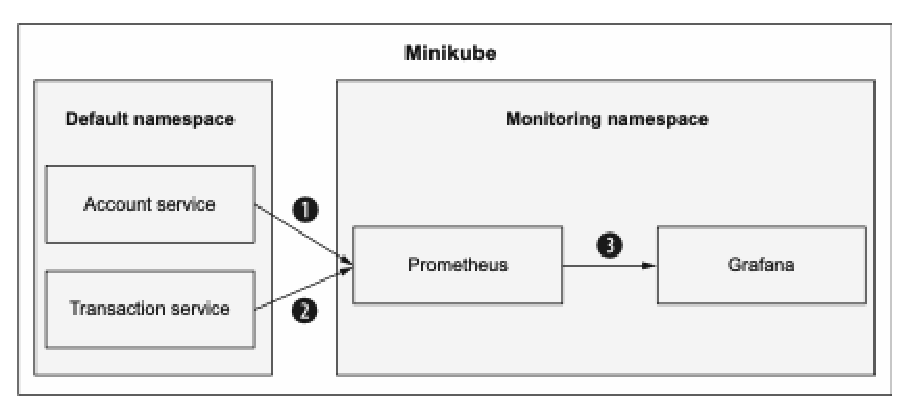
\includegraphics[width=.7\textwidth]{images/4-tracing_metrics/prom graf flow.pdf}
    \caption{Prometheus-Grafana Flow.}
    \label{fig:pr_gr_flow}
\end{figure}

Come dette nella Sezione~\ref{sec:prometheus} l'installazione all'interno del cluster Minikube è stata fatta con il chart di Helm \textit{kube-prometheus-stack}~\cite{prometheus_stack}, che comprende sia Prometheus che Grafana.